%% introduction.tex
%%
%% Introduction to the course ``Economic aspects'' of the
%%   Official Master on Libre Software (URJC)
%%   http://master.libresoft.es

%%---------------------------------------------------------------------
%%---------------------------------------------------------------------
\section{Linear models in R}

%%---------------------------------------------------------------

\begin{frame}
\frametitle{Linear models}

The goal is to fit a model characterizing the behavior of an \textbf{output} (response or dependant)
variable, according to one or several \textbf{input} (predictor, independent or explanatory) variables.

\end{frame}

%%---------------------------------------------------------------

\begin{frame}
\frametitle{Preparing your linear model}

\begin{itemize}
  \item Identify your response variable
  \item Identify the explanatory variable(s).
  \item Are the explanatory variables continuous, factors (categorical) or mixed?
  \item What's the type of your response variable (continuous, factor, count, proportion, binary, time at death, category)
\end{itemize}

\end{frame}

%%---------------------------------------------------------------

\begin{frame}
\frametitle{Available linear models}
\textbf{Explanatory variables}
\begin{itemize}
\item All continuous: Regression.
\item All categorical: Analysis of Variance (ANOVA).
\item Mixed: Analysis of Covariance (ANCOVA).
\end{itemize}

\end{frame}

%%---------------------------------------------------------------

\begin{frame}
\frametitle{Available linear models}

\textbf{Output variable}
\begin{itemize}
\item Continuous: Standard (simple/multivariate) regression, ANOVA, ANCOVA.
\item Proportion: Logistic regression.
\item Count: Log-linear models (Poisson regression).
\item Binary: Binary logistic analysis.
\item Time at death: Survival analysis.
\end{itemize}

\end{frame}

%%---------------------------------------------------------------------
\subsection{Simple regression}

%%---------------------------------------------------------------

\begin{frame}
\frametitle{lm() function in R}

\begin{itemize}
 \item $lm(Formula, data = dataset)$ let us fit linear models to data
 \item We need to write the adequate \textit{formula} to build the model.
 \item $lm(y ~ x0 + x1 + x2 + x3, data = my-data-frame)$
 \item We can express more complicated interactions (still linear models):
 \item $lm(y ~ x0 + x1*x2 + log(x3), data = my-data-frame)$

\end{itemize}
\end{frame}

%%---------------------------------------------------------------

% \begin{frame}
% \frametitle{The growth of libre software (2)}
% 
% 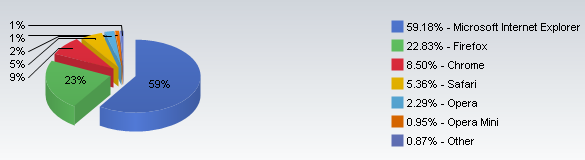
\includegraphics[height=3.5cm]{webbrowsers-share-2010-10}
% 
% \begin{flushright}
% Net Market Share Report, October 2010 \\
% {\small \url{http://www.netmarketshare.com/}}
% \end{flushright}
% \end{frame}

%%---------------------------------------------------------------------
\subsection{References}

%%---------------------------------------------------------------

\begin{frame}
\frametitle{References on linear models}

\begin{itemize}
 \item \small [Faraway, 2005] Faraway, J. (2005) Linear models with R. CRC Press.
 \item \small [Crawley, 2007] Crawley, M. J. The R book. Wiley.
 \item \small [Kutner et al., 2004] Kutner, M., Nachtsheim, C., Neter, J. and Li, W. (2004).
Applied Linear Statistical Models. McGraw-Hill.

 \end{itemize}
\end{frame}

%%---------------------------------------------------------------

\begin{frame}
\frametitle{Linear models with R}

\begin{itemize}
 \item \small [Faraway, 2002] Faraway, J. Practical Regression and Anova Using R.
 \url{http://cran.r-project.org/doc/contrib/Faraway-PRA.pdf}

 \item \small [Faraway, 2002] Faraway, J. Introduction to Probability and Statistics Using R.
 \url{http://www.lulu.com/items/volume_68/8123000/8123594/3/print/IPSUR.pdf}

 \end{itemize}
\end{frame}

%%---------------------------------------------------------------
